Dieser Abschnitt beschreibt den Entwicklungsprozess, welchen wir im Laufe des Projektes durchlaufen haben, um ein komplettes Spiel in Processing zu erstellen.

\subsection{Erste Schritte in Processing}\label{subsec:erste-schritte}
Da unsere Gruppe erst wenig Erfahrung mit Processing hatte, haben wir zunächst in das Framework eingearbeitet. Es wurden einzelne kurze Programme erstellt, welche Funktionen wie dem Darstellen mehrere Quadrate in Processing erklärten.

\subsection{Umsetzung in 2D}\label{subsec:umsetzung-in-2D}
Nachdem wir genug Grundwissen über Processing hatten, haben wir mit der Entwicklung des Spiels in 2D angefangen. Dies hatte den Vorteil, dass wir die Grundmechaniken in einer einfacheren Umgebung umsetzen konnten, bevor wir in 3D übergingen.

Java ist eine objektorientierte Sprache. Deshalb wurde der Aufbau der Dateien auch objektorientiert geplant. Insgesamt wurden drei zusätzliche Klassen, zur Hauptklasse, erstellt. Eine Klasse kümmert sich um die Logik und Darstellung des Labyrinths. Eine Klasse kümmert sich um die Steuerung und Darstellung des Spielcharakters und die letzte Klasse, hilft bei der Berechnung, ob eine Kollision zwischen dem Charakter und dem Labyrinth auftritt. Gesteuert wird dies alles von der Hauptklasse, welche auch die Instanz von Processing besitzt.

Da es am Anfang noch keine funktionierende Schnittstelle zu unserem Backend und den damit verbundenen Generator für Labyrinthe gab, haben wir ein Labyrinth mit komplett zufälliger Verteilung generiert.
Mit diesem simplen Aufbau konnten wir schon mit der Umsetzung der einzelnen Klassen beginnen. Erst wurde das Labyrinth dargestellt, dann wurde der Spielcharakter hinzugefügt. Nachdem eine einfache Steuerung in alle Richtungen funktioniert hatte, haben wir uns um die Kollision gekümmert, damit man nicht einfach durch die Wände laufen kann.

\begin{figure}[hbtp!]
    \centering
    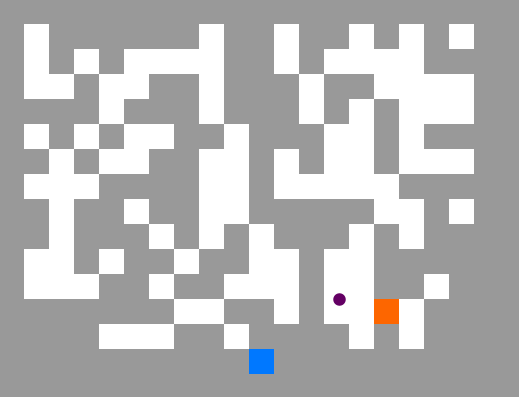
\includegraphics[width=\paperwidth-6in]{../assets/img/Fr2DTopDownRandom.PNG}
    \caption{Ein 2D Labyrinth mit zufällig plazierten Wänden}
    \label{fig:Fr2DTopDownRandom}
\end{figure}
Als Nächstes wurde die erste Schnittstelle für generierte Labyrinthe hinzugefügt, ein einfaches Auslesen einer JSON Datei, welche das Labyrinth in einem Grid gespeichert hat.
Da die meisten Mechaniken schon zuvor umgesetzt wurden, war das Spiel damit in dem ersten komplett spielbaren Stand.

\begin{figure}[hbtp!]
    \centering
    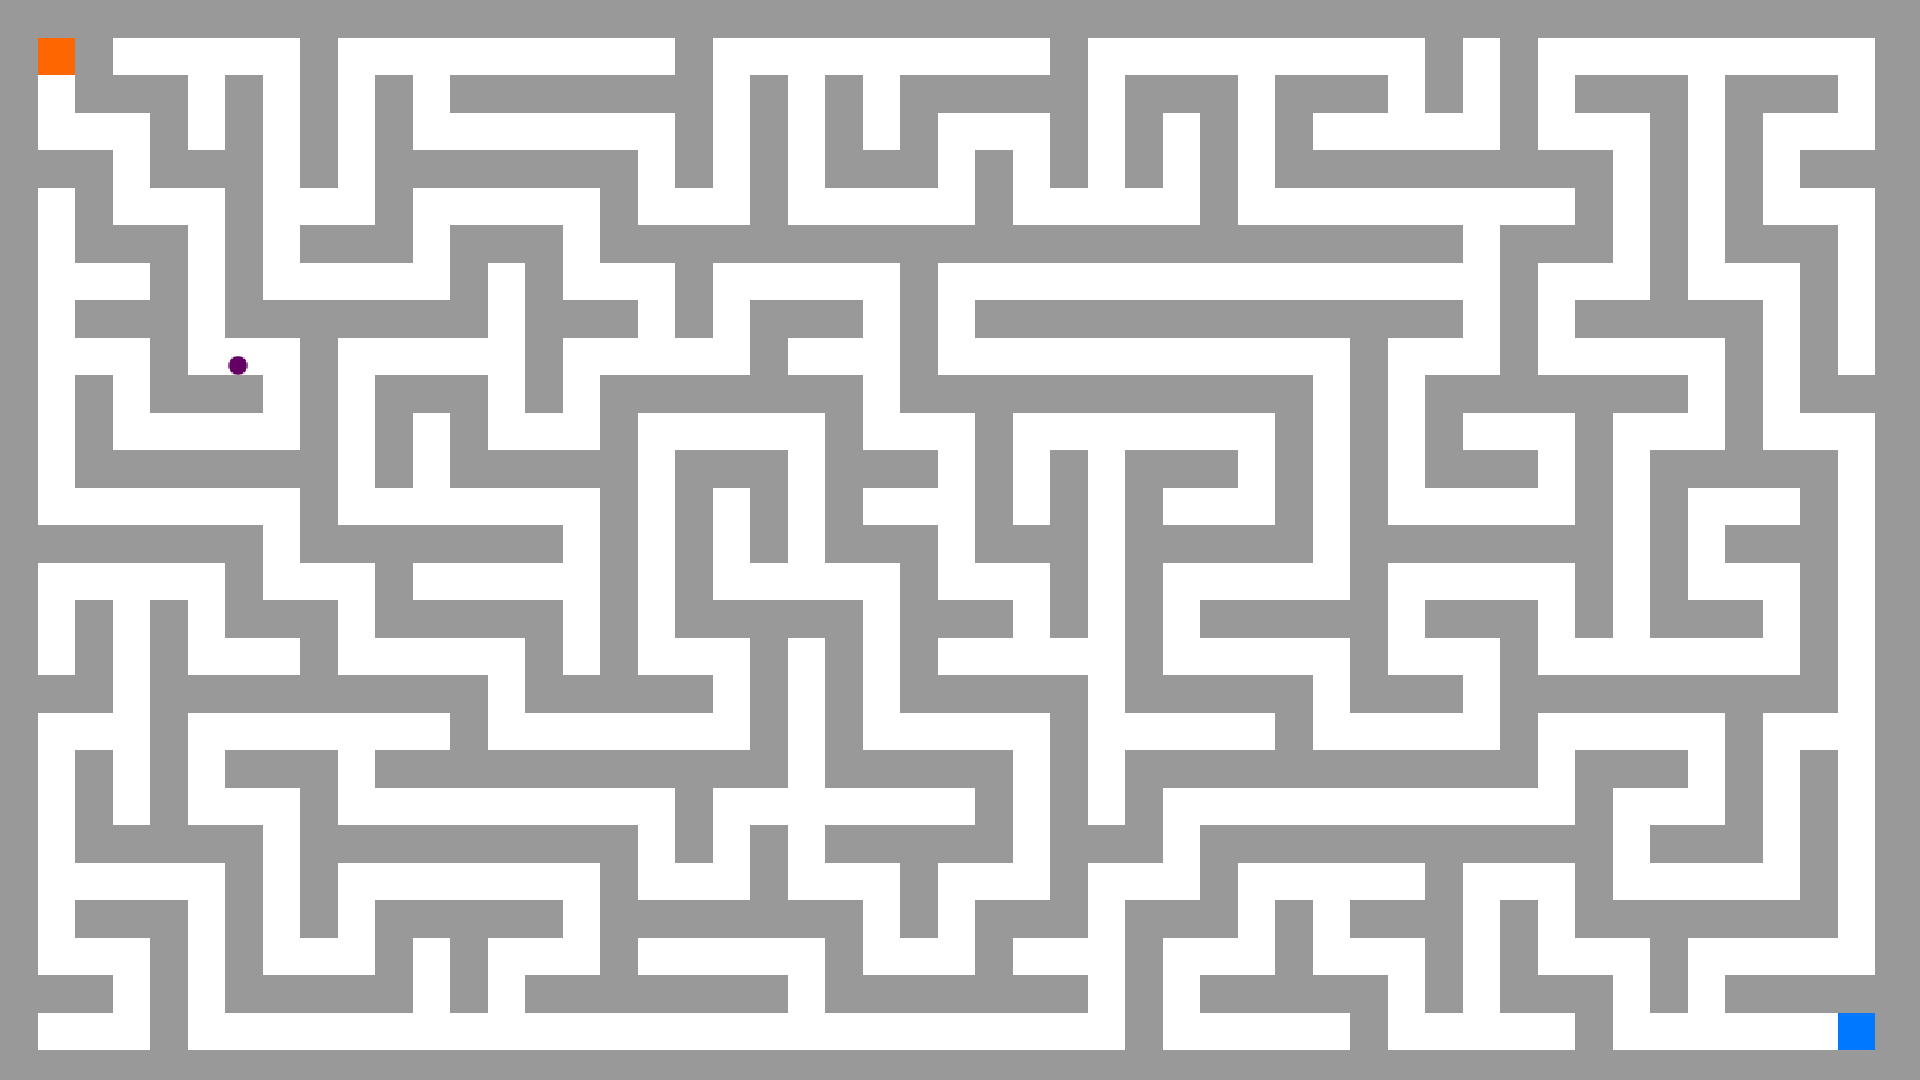
\includegraphics[width=\paperwidth-3in]{../assets/img/Fr2DTopDown.PNG}
    \caption{Darstellung des Labyrinthes in 2D}
    \label{fig:Fr2DTopDown}
\end{figure}

\subsection{Umsetzung in 3D}\label{subsec:umsetzung-in-3D}
Nachdem das Spiel in 2D funktionierte, sind wir auf 3D umgestiegen. Da, wie zuvor schon erwähnt, Java eine objektorientierte Sprache ist, haben wir möglichst viel Code der 2D Klassen vererbt und im Nachhinein angepasst.
Das Umsetzen in 3D war für uns besonders interessant, da wir bislang noch nichts in 3D gemacht haben. Deshalb haben wir wieder zunächst die Dokumentationen und Tutorials von Processing durchlaufen, um zu verstehen, wie genau Processing 3D umsetzt. Es stellte sich heraus, dass das Erstellen von Körper in 3D vergleichsweise einfach war, nachdem wir vieles von der 2D Umsetzung übernehmen konnten. Jedoch muss man für die Kamera sehr viel selbst berechnen, da einem nur wenig abgenommen wird. Generell war die Kamerasteuerung einer der größten Hürden in der Umsetzung der 3D-Ansichten.
Es wurden 2 Ansichten umgesetzt, wobei wir erst uns auf eine Top-Down Ansicht fokussiert haben. Dies lag unter anderem daran, dass die Steuerung des Spielcharakters der 2D Ansicht ähnelte. Bei einer Top-Down Ansicht, sieht man ähnlich, wie bei einer 2D Ansicht von oben auf das Spielfeld. Teilweise wird dies auch gerne als Vogelperspektive bezeichnet, da die Kamera und damit der Spieler wie ein Vogel von oben schaut.

\begin{figure}[hbtp!]
    \centering
    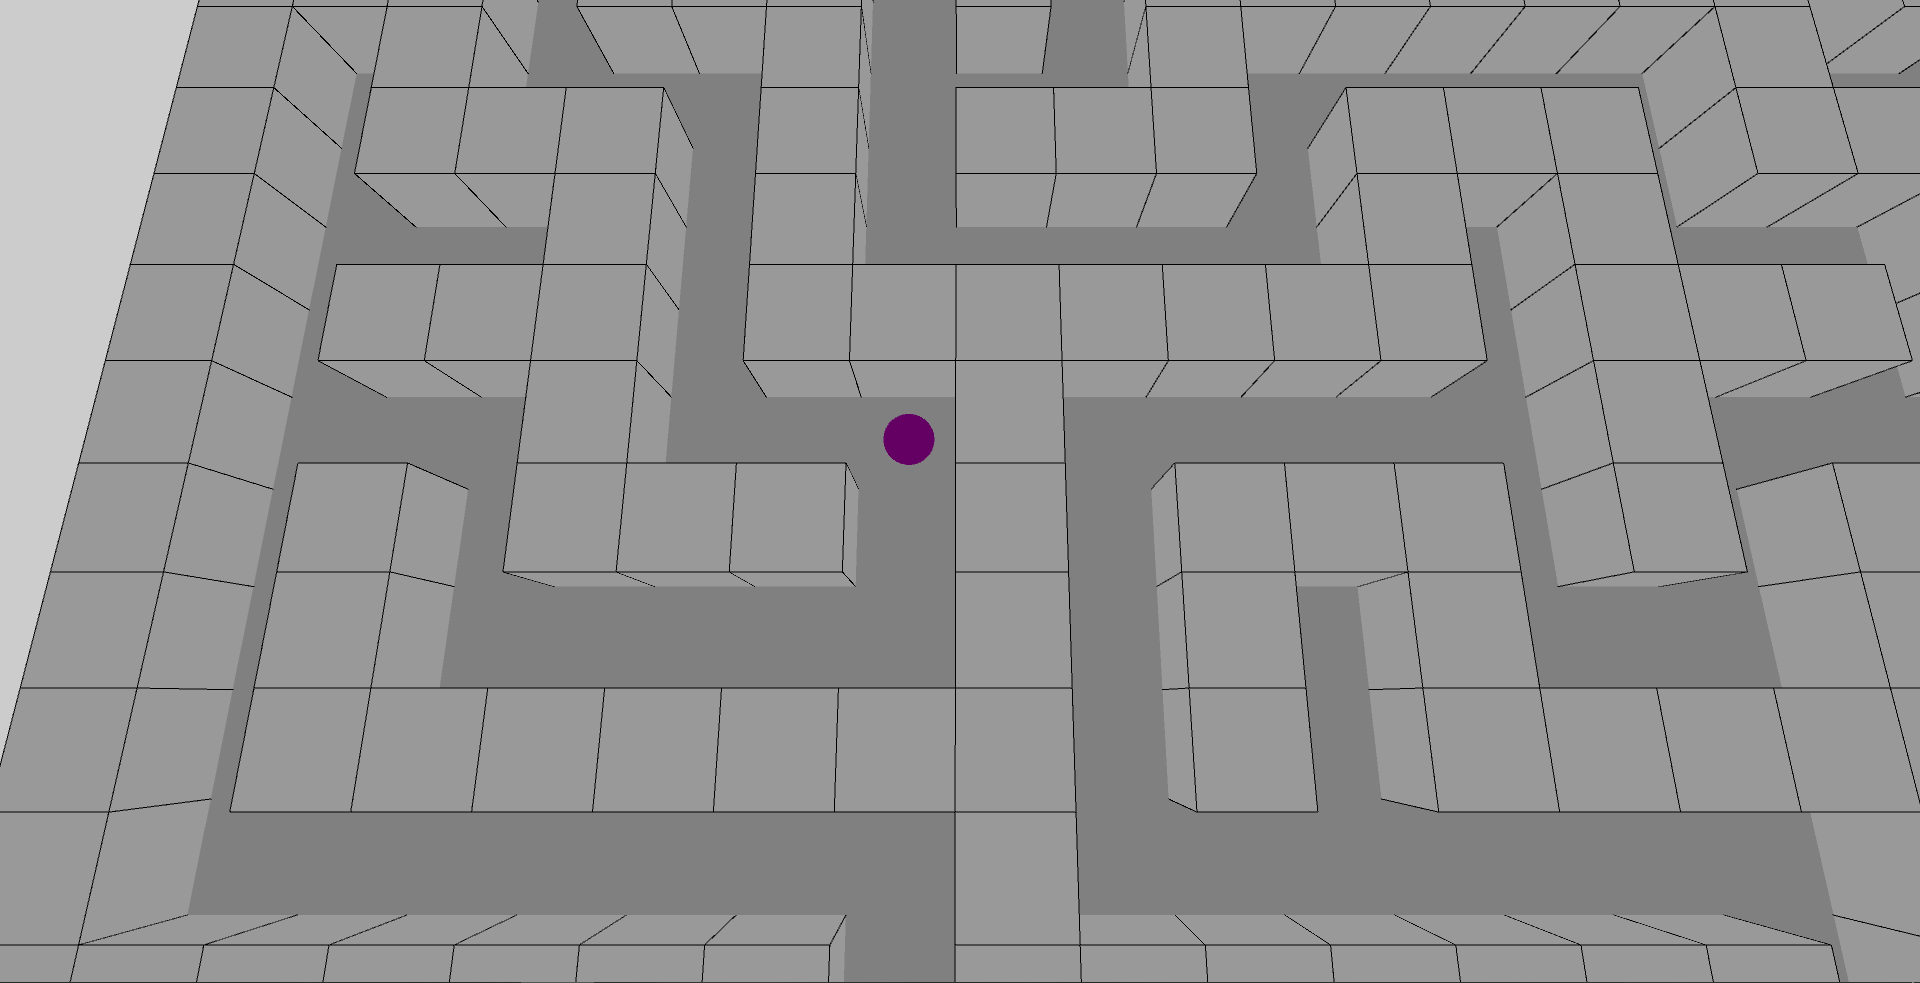
\includegraphics[width=\paperwidth-3in]{../assets/img/Fr3DTopDown.PNG}
    \caption{Erste Darstellung des Labyrinthes in 3D}
    \label{fig:Fr3DTopDown}
\end{figure}

Wie man auf Bild~\ref{fig:Fr3DTopDown} erkennen kann, war die Spielwelt sehr einfarbig. Deshalb erkundigten wir uns, wie man Texturen in 3D einfügt. Dabei lernten wir, dass die Standardfunktion für einen einfachen Würfel keine Möglichkeiten für Texturen gaben. Als Lösung haben wir stattdessen eigenen Würfel mithilfe von kombinierten 2D Flächen erstellt. Diese einzelnen Flächen kann man einfach mit einer Textur versehen, die als ganzes die Wände unseres Labyrinthes darstellten. Zusätzlich fügten wir einfache Lichtquellen ein, um dem Spiel etwas mehr Abwechslung zu bieten.

\begin{figure}[hbtp!]
    \centering
    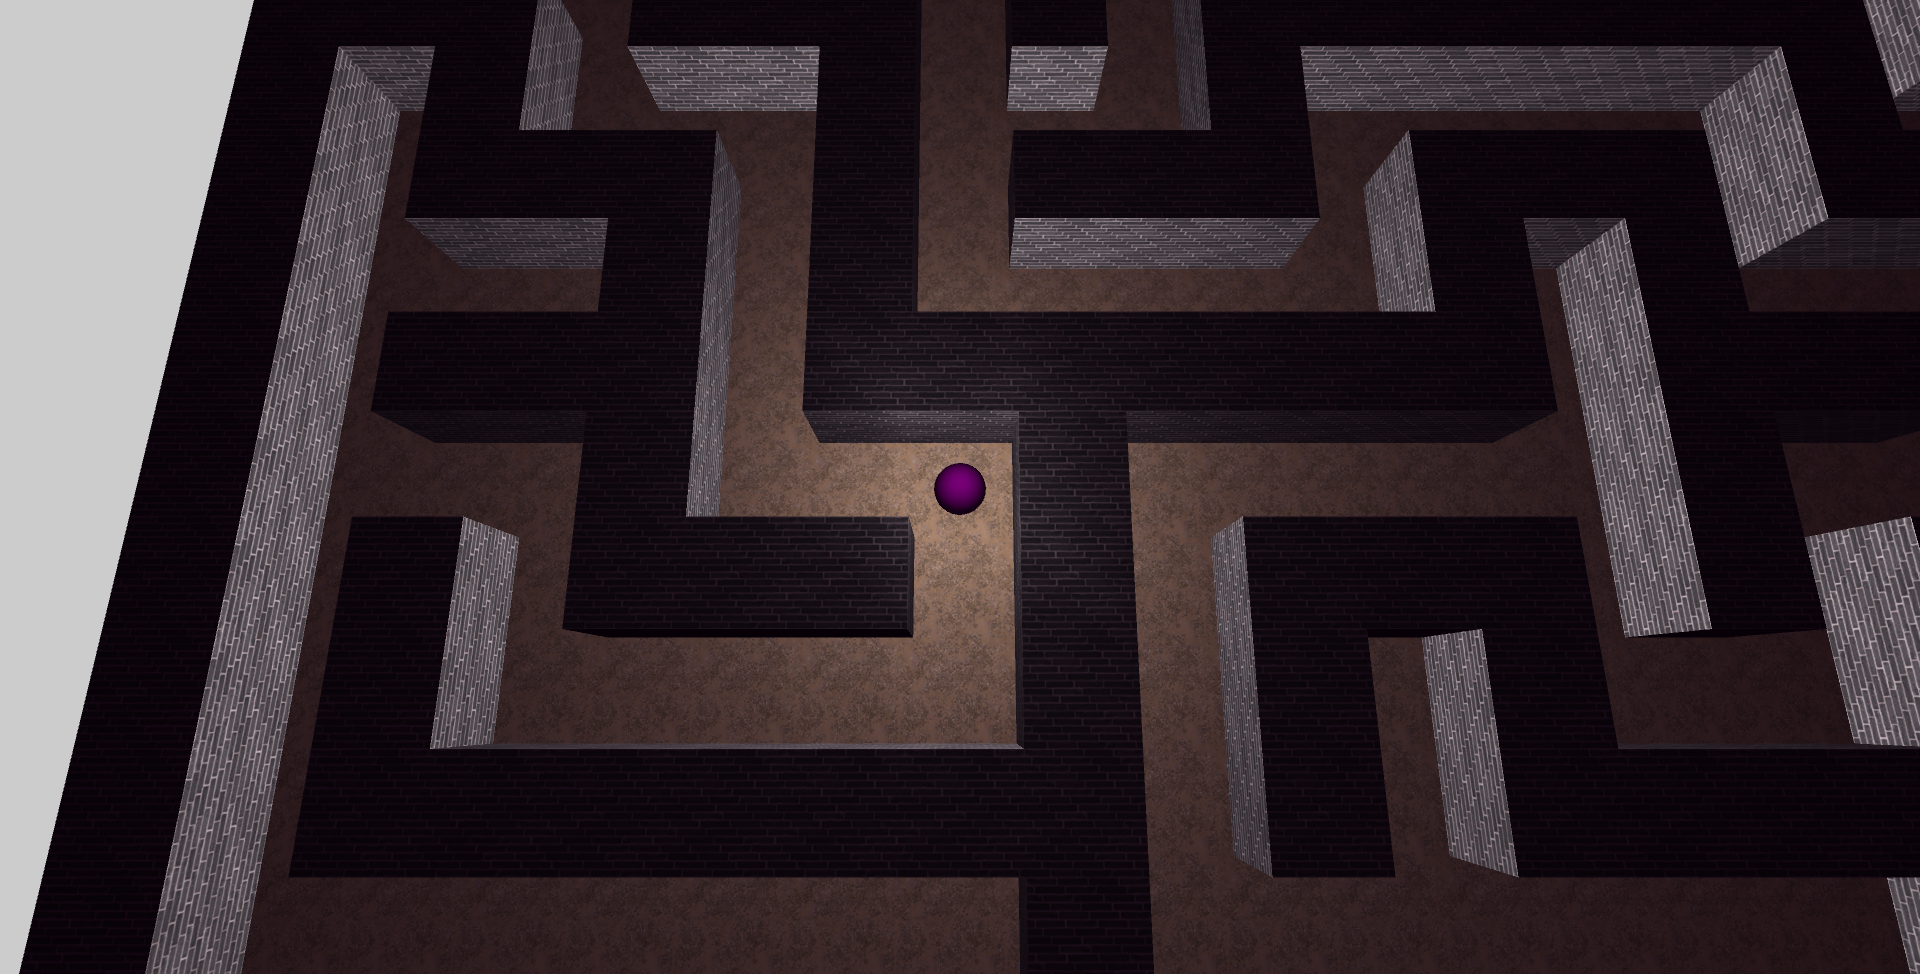
\includegraphics[width=\paperwidth-3in]{../assets/img/Fr3DTopDownTexture.PNG}
    \caption{Darstellung des Labyrinthes in 3D mit Texture und Licht}
    \label{fig:Fr3DTopDownTexture}
\end{figure}

Als die Top-Down 3D Ansicht unseren Wünschen entsprach, kümmerten wir uns um eine First-Person 3D Ansicht. Mit einer First-Person Ansicht meint man eine Ansicht, welche einem die Perspektive des Spielers selbst zeigt. Im Falle unseres Labyrinthes bedeutet dies also, dass man selbst im Labyrinth steckt und nicht einfach über die Wände schauen kann.
Da die Steuerung bislang rein über die 4 Himmelsrichtungen und den damit verbundenen Tasten gelang, mussten wir eine neue Steuerung für die First-Person Ansicht programmieren. Hierbei dreht man mithilfe der Maus den Spieler und die Kamera. Wenn man dann die Pfeiltasten zum Bewegen drückt, bewegt sich der Spieler relativ zur Kamera und nicht zu den Himmelsrichtungen. Dies alles war mit vielen Berechnungen verbunden, jedoch war das Ergebnis sehr zufriedenstellend.

\begin{figure}[hbtp!]
    \centering
    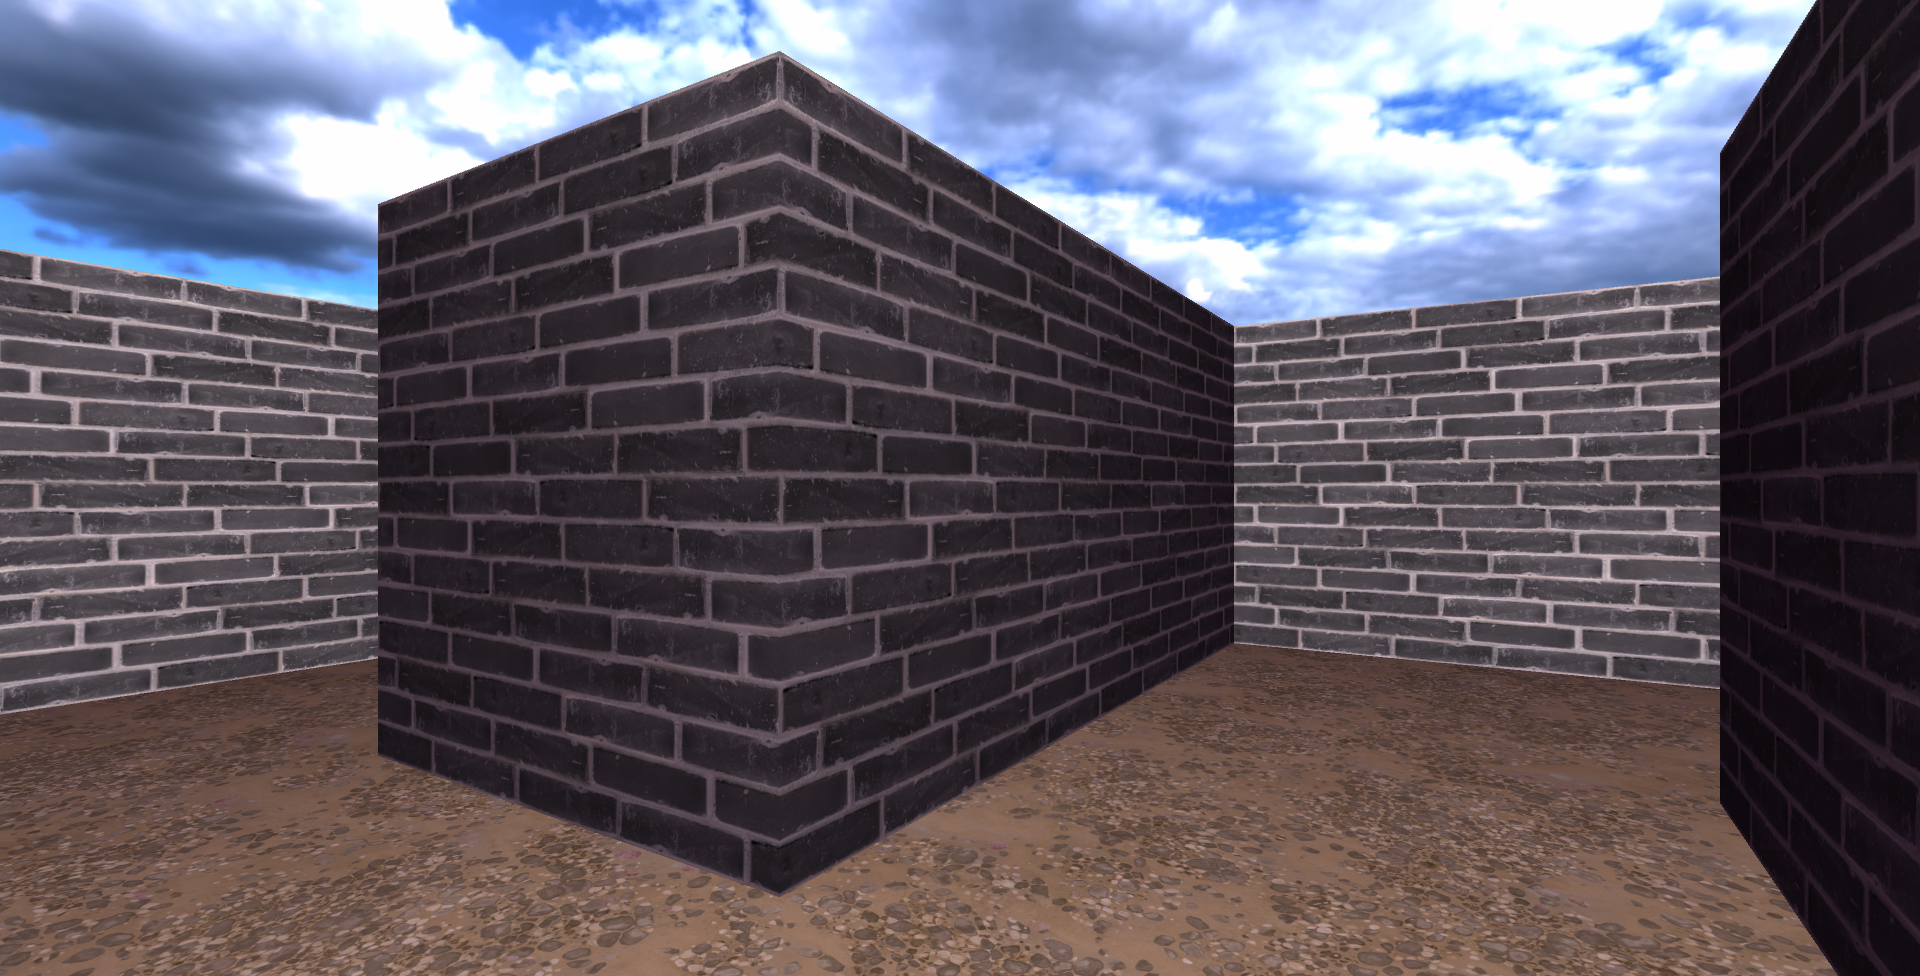
\includegraphics[width=\paperwidth-3in]{../assets/img/Fr3DFirstPersonTexture.PNG}
    \caption{Darstellung des Labyrinthes in 3D mit Texture und Licht}
    \label{fig:Fr3DFirstPersonTexture}
\end{figure}

Zu guter Letzt wurden einige Optimierungen an der Darstellung durchgeführt. Teile des Labyrinthes, welche sich außerhalb des Blickfeldes befinden, werden nicht mehr beachtet, was die Leistung enorm vergrößerte. Der Laptop, auf welchem das Spiel die meiste Zeit programmiert und getestet wurde, konnte zunächst nur Spielflächen mit einer Größe von 50 mal 30 flüssig darstellen. Nach der Optimierung hatte der Laptop auch mit Spielflächen von über 256 mal 256 keine Probleme mehr. 